\documentclass[a4paper,11pt]{article}
\usepackage[utf8]{inputenc}
\usepackage[T1]{fontenc}
\usepackage[french]{babel}
\usepackage{geometry}
\geometry{margin=2cm, top=2.5cm, bottom=2.5cm}
\usepackage{xcolor}
\usepackage{tikz}
\usepackage{graphicx}
\usepackage{booktabs}
\usepackage{array}
\usepackage{longtable}
\usepackage{hyperref}
\usepackage{enumitem}
\usepackage{fancyhdr}
\usepackage{titlesec}
\usepackage{mdframed}
\usepackage{listings}
\usepackage{tcolorbox}
\tcbuselibrary{skins, breakable}

%% ── Palette couleurs BNM ──────────────────────────────────────────────────────
\definecolor{bnmblue}{rgb}{0,0.2,0.4}
\definecolor{bnmlightblue}{rgb}{0,0.4,0.702}
\definecolor{bnmred}{rgb}{0.753,0,0}
\definecolor{bnmgreen}{rgb}{0,0.502,0}
\definecolor{bnmorange}{rgb}{0.980,0.922,0.922}
\definecolor{bnmgray}{rgb}{0.314,0.314,0.314}
\definecolor{bnmlightgray}{rgb}{0.961,0.961,0.961}
\definecolor{bnmwarning}{rgb}{0.980,0.549,0}
\definecolor{mysqlblue}{RGB}{0,117,180}
\definecolor{clickgreen}{RGB}{0,128,64}
\definecolor{plenigedpurple}{RGB}{102,0,153}
\definecolor{zoneblue}{RGB}{220,235,250}
\definecolor{zonegreen}{RGB}{210,240,220}

%% ── En-tête / Pied de page ────────────────────────────────────────────────────
\pagestyle{fancy}
\fancyhf{}
\fancyhead[L]{\textbf{\textcolor{bnmblue}{BNM}}}
\fancyhead[R]{\textcolor{bnmgray}{\small Blueprint DR MySQL v1.0 — CONFIDENTIEL}}
\fancyfoot[C]{\textcolor{bnmgray}{\small \thepage}}
\fancyfoot[R]{\textcolor{bnmgray}{\small Usage Interne Uniquement}}
\renewcommand{\headrulewidth}{0.4pt}
\renewcommand{\headrule}{\hbox to\headwidth{\color{bnmblue}\leaders\hrule height \headrulewidth\hfill}}

%% ── Style des titres ──────────────────────────────────────────────────────────
\titleformat{\section}
  {\large\bfseries\color{bnmblue}}
  {\thesection}{1em}{}
  [\vspace{-0.5em}\textcolor{bnmblue}{\rule{\linewidth}{0.8pt}}]

\titleformat{\subsection}
  {\normalsize\bfseries\color{bnmlightblue}}
  {\thesubsection}{1em}{}

\titleformat{\subsubsection}
  {\normalsize\bfseries\color{bnmgray}}
  {\thesubsubsection}{1em}{}

%% ── Boîtes colorées ───────────────────────────────────────────────────────────
\newenvironment{alertbox}[1][Attention]{%
  \begin{tcolorbox}[colback=bnmorange, colframe=bnmred, fonttitle=\bfseries, title=#1]
}{%
  \end{tcolorbox}
}

\newenvironment{infobox}[1][Information]{%
  \begin{tcolorbox}[colback=zoneblue, colframe=bnmlightblue, fonttitle=\bfseries, title=#1]
}{%
  \end{tcolorbox}
}

\newenvironment{successbox}[1][Succès]{%
  \begin{tcolorbox}[colback=zonegreen, colframe=bnmgreen, fonttitle=\bfseries, title=#1]
}{%
  \end{tcolorbox}
}

%% ── Style code bash ───────────────────────────────────────────────────────────
\lstset{
  basicstyle=\small\ttfamily,
  backgroundcolor=\color{bnmlightgray},
  frame=single,
  rulecolor=\color{bnmgray},
  keywordstyle=\color{mysqlblue}\bfseries,
  commentstyle=\color{bnmgreen},
  stringstyle=\color{bnmred},
  breaklines=true,
  postbreak=\mbox{\textcolor{red}{$\hookrightarrow$}\space},
  showstringspaces=false
}

%% ══════════════════════════════════════════════════════════════════════════════
\begin{document}

%% ── PAGE DE TITRE ─────────────────────────────────────────────────────────────
\begin{tikzpicture}[remember picture, overlay]
  \fill[bnmblue] (current page.north west) rectangle ([yshift=-5cm]current page.north east);
  \fill[bnmlightblue] ([yshift=-5cm]current page.north west) rectangle ([yshift=-6.5cm]current page.north east);
\end{tikzpicture}

\vspace*{1cm}
\begin{center}
  {\Huge\bfseries\textcolor{white}{Blueprint DR MySQL}}\\[0.5em]
  {\large\textcolor{white!80!bnmlightblue}{Implémentation Disaster Recovery}}\\[0.3em]
  {\large\textcolor{white!80!bnmlightblue}{Click \& Pleniged — Architecture \& Plan d'Exécution}}\\[2.5cm]
\end{center}

\begin{center}
\begin{tabular}{ll}
  \textbf{\textcolor{bnmblue}{Version}}   & 1.0\\
  \textbf{\textcolor{bnmblue}{Date}}      & 22 Mars 2026\\
  \textbf{\textcolor{bnmblue}{Statut}}    & \textcolor{bnmgreen}{\textbf{Actif — Document de Référence}}\\
  \textbf{\textcolor{bnmblue}{Go-Live}}   & \textcolor{bnmred}{\textbf{fin Avril 2026}}\\
  \textbf{\textcolor{bnmblue}{Titulaires}}& Ing. Betah Lab \& Dr. Fatimetou Abdou\\
  \textbf{\textcolor{bnmblue}{Stagiaires}}& Ethmane Mahmoud Ethmane (Track Oracle)\\
                                           & Ahmed Abd Dayem Ahmed Bouha (Track MySQL/FS)\\
  \textbf{\textcolor{bnmblue}{Direction}} & Direction Système d'Information — BNM\\
\end{tabular}
\end{center}

\vspace{1cm}
\begin{center}
  \textcolor{bnmgray}{\small Document de référence unique du projet DR MySQL. Toute modification validée par le Team Lead uniquement.}
\end{center}

\newpage
\tableofcontents
\newpage

%% ══════════════════════════════════════════════════════════════════════════════
\section{Contexte et Objectifs}

\begin{alertbox}[Situation Actuelle]
Aucune stratégie de réplication ou de reprise après sinistre n'existe actuellement pour les systèmes \textbf{Click} (MySQL 8.0 / Ubuntu) et \textbf{Pleniged} (MySQL 8.0 / Windows + FileSystem 4~TB). En cas de panne majeure, la perte totale et irréversible des données est possible.
\end{alertbox}

\vspace{0.5em}

\begin{successbox}[Objectifs du Projet]
\begin{itemize}[noitemsep]
  \item RPO $\approx$ 0 pour les bases de données Click et Pleniged via réplication semi-synchrone.
  \item RTO $<$ 2 heures pour le basculement en Zone 2 (site secondaire).
  \item RTO $<$ 60 minutes pour Pleniged FS via synchronisation DRBD/rsync nocturne.
  \item Mise en œuvre avec Go-Live cible : \textbf{fin Avril 2026}.
\end{itemize}
\end{successbox}

%% ══════════════════════════════════════════════════════════════════════════════
\section{Architecture DR — Vue d'Ensemble}

\begin{center}
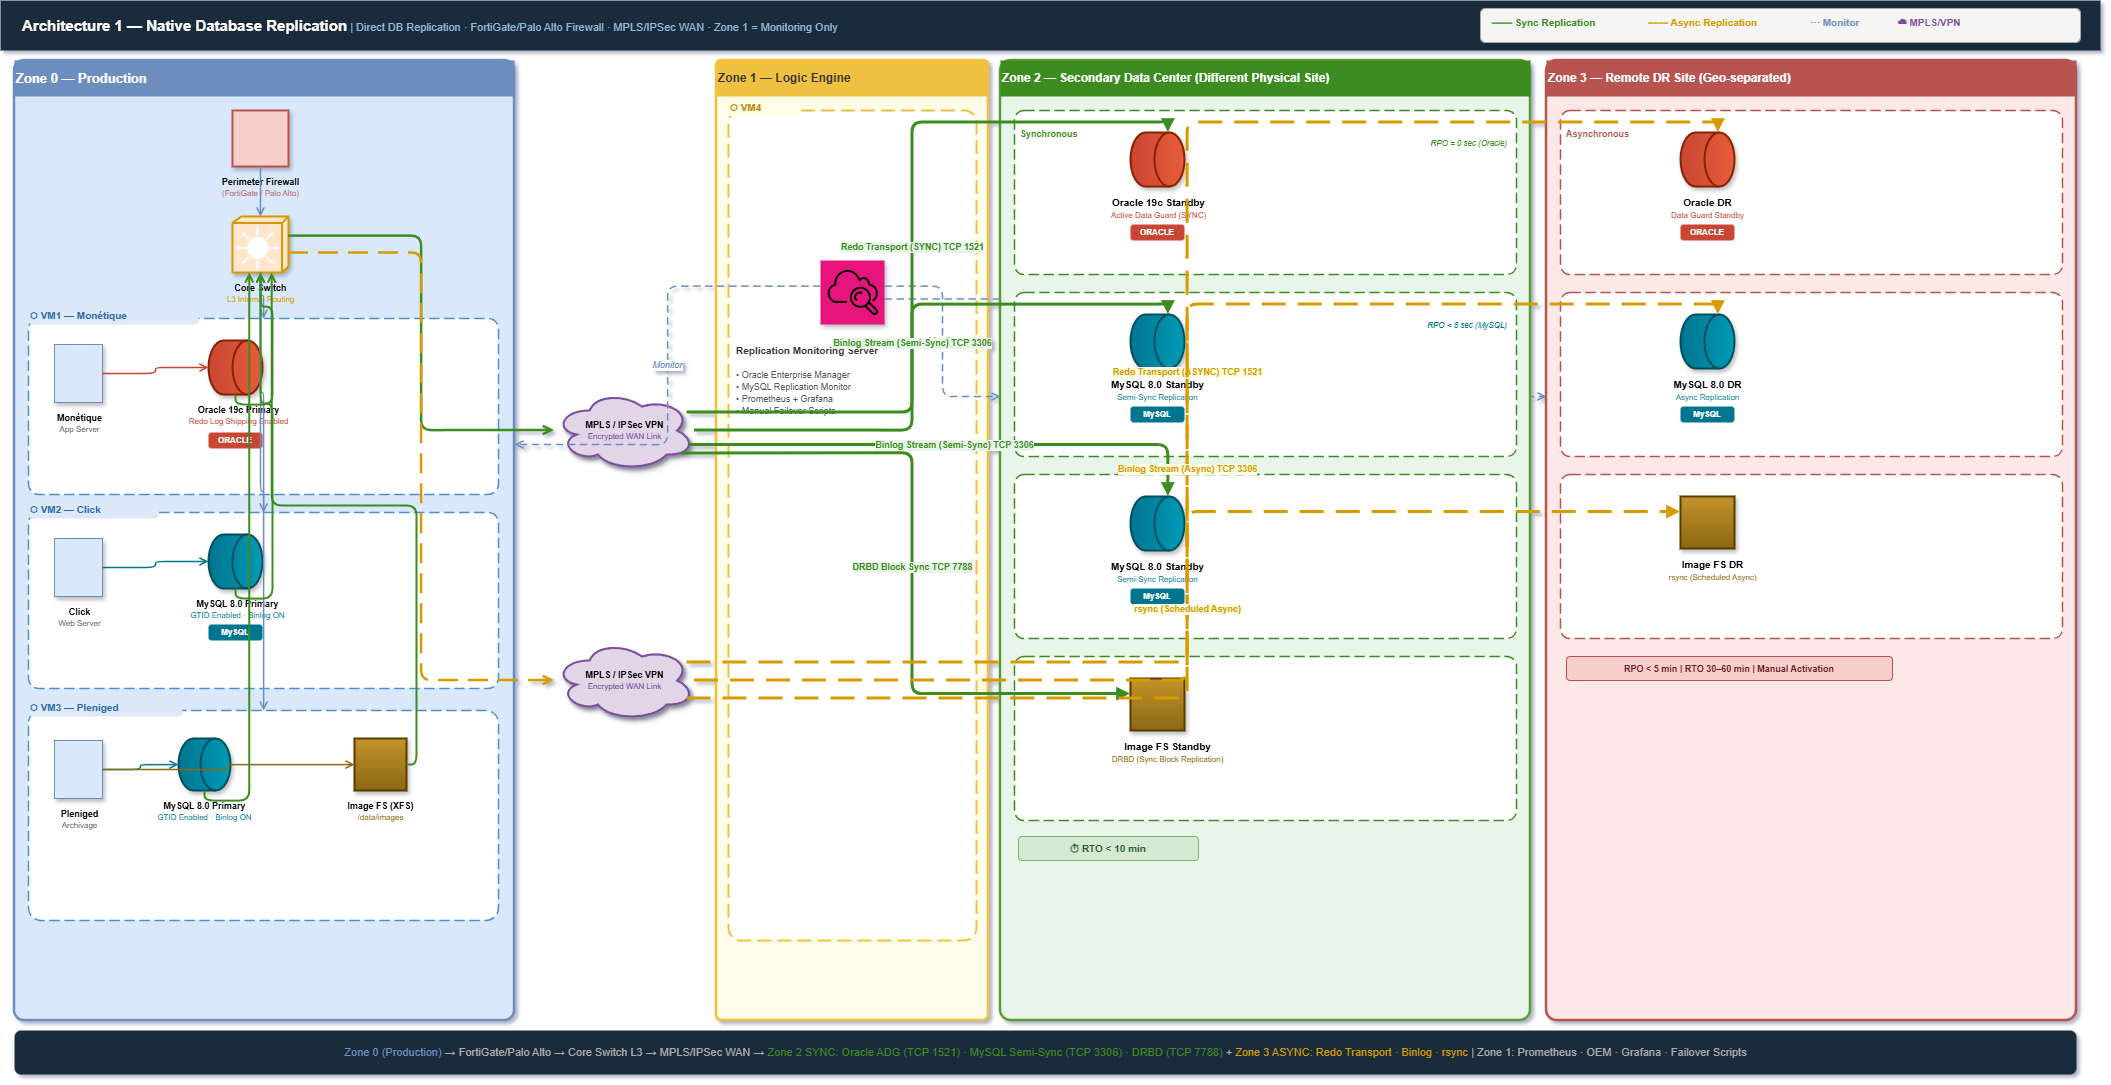
\includegraphics[width=\linewidth]{latexImage_f849d4e5944aecb3c83fcc92746aac90.png}
\end{center}
\begin{center}
  \textit{\small Figure 1 : Architecture DR Native — Zone 0 (Production) vers Zone 2 (DR) et Zone 3 (DR Distant)}
\end{center}

\vspace{1em}

\begin{infobox}[Lecture du Schéma]
\begin{itemize}[noitemsep]
  \item \textcolor{bnmgreen}{\textbf{Ligne verte :}} Réplication Semi-Synchrone (RPO = 0) vers Zone 2.
  \item \textcolor{bnmwarning}{\textbf{Ligne orange :}} Réplication Asynchrone (RPO $\approx$ 0) vers Zone 3.
  \item \textbf{Architecture Double-Instance} : Zone 2 et Zone 3 hébergent chacune Click (:3306) et Pleniged (:3307).
  \item \textbf{Zone 2} : Centre secondaire (Hot Standby), réplication semi-synchrone.
  \item \textbf{Zone 3} : Centre tertiaire (Warm Standby), réplication asynchrone parallèle.
\end{itemize}
\end{infobox}

%% ══════════════════════════════════════════════════════════════════════════════
\section{Inventaire des Systèmes MySQL}

\begin{table}[h!]
\centering
\renewcommand{\arraystretch}{1.4}
\begin{tabular}{|>{\bfseries}l|l|l|l|l|}
\hline
\rowcolor{bnmblue}\textcolor{white}{Système} & \textcolor{white}{VM} & \textcolor{white}{OS} & \textcolor{white}{RAM / CPU} & \textcolor{white}{Taille DB} \\
\hline
Click & VM2 & Ubuntu Linux & 32 GB / 16 cœurs & $\sim$0,1 GB \\
\hline
\rowcolor{bnmlightgray}
Pleniged DB & VM3 & Windows Server & 32 GB / 16 cœurs & $\sim$32 GB \\
\hline
Pleniged FS & VM3 & Windows Server & — & $\sim$4 TB \\
\hline
\end{tabular}
\caption{Inventaire des serveurs MySQL de production — Zone 0}
\end{table}

%% ══════════════════════════════════════════════════════════════════════════════
\section{Stack Technologique MySQL DR}

\begin{table}[h!]
\centering
\renewcommand{\arraystretch}{1.4}
\begin{tabular}{|>{\bfseries}l|l|l|l|}
\hline
\rowcolor{bnmblue}\textcolor{white}{Conteneur} & \textcolor{white}{Site Source} & \textcolor{white}{Site DR} & \textcolor{white}{Port DR} \\
\hline
mysql-click & 192.168.1.241 & Zone 2 / Zone 3 & TCP 3306 \\
\hline
\rowcolor{bnmlightgray}
mysql-pleniged & 10.168.2.34 & Zone 2 / Zone 3 & TCP 3307 \\
\hline
\end{tabular}
\caption{Allocation des ports pour l'architecture Double-Instance}
\end{table}

%% ══════════════════════════════════════════════════════════════════════════════
\section{Objectifs RTO / RPO}

\begin{table}[h!]
\centering
\renewcommand{\arraystretch}{1.4}
\begin{tabular}{|>{\bfseries}l|l|l|l|}
\hline
\rowcolor{bnmblue}\textcolor{white}{Système} & \textcolor{white}{RPO} & \textcolor{white}{RTO} & \textcolor{white}{Méthode} \\
\hline
Click (BDD) & $\approx$ 0 & $<$ 2 h & MySQL Semi-Sync vers Zone 2 \\
\hline
\rowcolor{bnmlightgray}
Pleniged DB & $\approx$ 0 & $<$ 2 h & MySQL Semi-Sync vers Zone 2 \\
\hline
Pleniged FS & $<$ 24 h & $<$ 24 h & rsync nocturne vers Zone 2 \\
\hline
\end{tabular}
\caption{Objectifs RTO/RPO validés pour les systèmes MySQL}
\end{table}

%% ══════════════════════════════════════════════════════════════════════════════
\section{Plan d'Implémentation Détaillé}

\subsection{Prérequis — Ce Dont Nous Avons Besoin}

\begin{infobox}[Prérequis Infrastructure]
\begin{enumerate}[noitemsep]
  \item \textbf{VMs DR (Zone 2 \& 3)} : Serveurs Ubuntu 22.04 avec Docker et Docker-Compose.
  \item \textbf{Règles réseau} : Ouverture TCP 3306 (Click) et TCP 3307 (Pleniged) entre Zones.
  \item \textbf{Isolation} : Utilisation de volumes Docker séparés pour Click et Pleniged.
  \item \textbf{Monitoring} : Installation de mysqld\_exporter sur les ports 9104 et 9105.
\end{enumerate}
\end{infobox}

%% ── Épique 1 ──────────────────────────────────────────────────────────────────
\subsection{Épique 1 : Préparation de l'Infrastructure DR}

\subsubsection{Tâche 1.1 — Provisionner la VM DR pour Click (Ubuntu)}

\textbf{Responsable :} Ahmed Abd Dayem Ahmed Bouha \quad \textbf{Durée estimée :} 1 jour

\begin{itemize}[noitemsep]
  \item Créer une VM Ubuntu Linux (32 GB RAM, 16 vCPUs, 500 GB disque).
  \item Vérifier la connectivité réseau avec la VM2 de production (ping, traceroute).
  \item Appliquer les politiques de sécurité BNM (pare-feu, SSH par clé uniquement).
\end{itemize}

\begin{lstlisting}[language=bash, caption={Vérification connectivité depuis VM DR vers VM2 production}]
# Depuis la VM DR Click (Zone 2)
ping -c 4 <IP_VM2_Production>
telnet <IP_VM2_Production> 3306
# Résultat attendu : connexion établie sur port 3306
\end{lstlisting}

\subsubsection{Tâche 1.2 — Provisionner la VM DR pour Pleniged (Windows)}

\textbf{Responsable :} Ahmed Abd Dayem Ahmed Bouha \quad \textbf{Durée estimée :} 1 jour

\begin{itemize}[noitemsep]
  \item Créer une VM Windows Server (32 GB RAM, 16 vCPUs, 10 TB stockage pour FS).
  \item Vérifier la connectivité réseau avec la VM3 de production (port 3306 et SSH).
  \item Monter le volume de stockage destiné à la réplication du FileSystem (4 TB+).
\end{itemize}

\subsubsection{Tâche 1.3 — Configuration des règles Réseau et Pare-feu}

\textbf{Responsable :} Ing. Betah Lab \quad \textbf{Durée estimée :} 0,5 jour

\begin{table}[h!]
\centering
\renewcommand{\arraystretch}{1.3}
\begin{tabular}{|l|l|l|l|}
\hline
\rowcolor{bnmblue}\textcolor{white}{Source} & \textcolor{white}{Destination} & \textcolor{white}{Port} & \textcolor{white}{Usage} \\
\hline
VM2 Production & VM DR Click & TCP 3306 & Réplication MySQL \\
\hline
\rowcolor{bnmlightgray}
VM3 Production & VM DR Pleniged & TCP 3306 & Réplication MySQL \\
\hline
VM3 Production & VM DR Pleniged & TCP 7788 & Sync DRBD \\
\hline
\rowcolor{bnmlightgray}
VM3 Production & VM DR Pleniged & TCP 22 (SSH) & rsync FS nocturne \\
\hline
\end{tabular}
\caption{Règles de pare-feu à ouvrir sur FortiGate/Palo Alto}
\end{table}

%% ── Épique 2 ──────────────────────────────────────────────────────────────────
\subsection{Épique 2 : Implémentation DR pour Click (Ubuntu / MySQL 8.0)}

\subsubsection{Tâche 2.1 — Installation MySQL 8.0 sur la VM DR Click}

\textbf{Responsable :} Ahmed Abd Dayem Ahmed Bouha \quad \textbf{Durée estimée :} 0,5 jour

\begin{lstlisting}[language=bash, caption={Installation MySQL 8.0 sur Ubuntu (VM DR Click)}]
# Mise à jour du système
sudo apt update && sudo apt upgrade -y

# Installation MySQL 8.0
sudo apt install -y mysql-server

# Vérification de la version
mysql --version
# Résultat attendu : mysql  Ver 8.0.xx for Linux

# Sécurisation initiale
sudo mysql_secure_installation
\end{lstlisting}

\subsubsection{Tâche 2.2 — Installation et configuration de Percona XtraBackup}

\textbf{Responsable :} Ahmed Abd Dayem Ahmed Bouha \quad \textbf{Durée estimée :} 0,5 jour

\begin{lstlisting}[language=bash, caption={Installation Percona XtraBackup sur le serveur primaire Click}]
# Sur VM2 Production (Production Primary) ET VM DR Click
wget https://repo.percona.com/apt/percona-release_latest.$(lsb_release -sc)_all.deb
sudo dpkg -i percona-release_latest.*.deb
sudo percona-release enable-only tools
sudo apt update
sudo apt install -y percona-xtrabackup-80

# Vérification
xtrabackup --version
\end{lstlisting}

\subsubsection{Tâche 2.3 — Sauvegarde complète initiale et restauration sur VM DR}

\textbf{Responsable :} Ahmed Abd Dayem Ahmed Bouha \quad \textbf{Durée estimée :} 1 jour

\begin{lstlisting}[language=bash, caption={Sauvegarde initiale sur le primaire Click et restauration en DR}]
##############################################
# ÉTAPE 1 : Sur VM2 Production (Primary)
##############################################
# Créer la sauvegarde physique complète
sudo xtrabackup --backup \
  --user=root --password=<MOT_DE_PASSE> \
  --target-dir=/data/backup/click_full_$(date +%F)

# Préparer la sauvegarde (apply-log)
sudo xtrabackup --prepare \
  --target-dir=/data/backup/click_full_$(date +%F)

# Transférer la sauvegarde vers le DR via SSH
rsync -avz --progress \
  /data/backup/click_full_$(date +%F)/ \
  ubuntu@<IP_DR_CLICK>:/data/restore/

##############################################
# ÉTAPE 2 : Sur VM DR Click
##############################################
# Arrêter MySQL si en cours d'exécution
sudo systemctl stop mysql

# Vider le répertoire de données MySQL
sudo rm -rf /var/lib/mysql/*

# Restaurer la sauvegarde
sudo xtrabackup --copy-back \
  --target-dir=/data/restore/click_full_*/

# Corriger les permissions
sudo chown -R mysql:mysql /var/lib/mysql

# Démarrer MySQL
sudo systemctl start mysql
sudo systemctl status mysql
\end{lstlisting}

\subsubsection{Tâche 2.4 — Configuration de la réplication semi-synchrone MySQL}

\textbf{Responsable :} Ahmed Abd Dayem Ahmed Bouha \quad \textbf{Durée estimée :} 1 jour

\begin{lstlisting}[language=bash, caption={Configuration réplication semi-synchrone sur VM2 Production (Primary)}]
##############################################
# Sur VM2 Production : activation semi-sync
##############################################
# Éditer /etc/mysql/mysql.conf.d/mysqld.cnf
[mysqld]
server-id           = 1
log_bin             = /var/log/mysql/mysql-bin.log
binlog_format       = ROW
gtid_mode           = ON
enforce_gtid_consistency = ON
plugin-load-add     = semisync_master.so
rpl_semi_sync_master_enabled = 1
rpl_semi_sync_master_timeout = 10000

# Redémarrer MySQL
sudo systemctl restart mysql

# Créer l'utilisateur de réplication
mysql -u root -p -e "
  CREATE USER 'replicateur'@'%' IDENTIFIED BY '<MOT_DE_PASSE_FORT>';
  GRANT REPLICATION SLAVE ON *.* TO 'replicateur'@'%';
  FLUSH PRIVILEGES;
"
\end{lstlisting}

\begin{lstlisting}[language=bash, caption={Configuration du serveur esclave (VM DR Click)}]
##############################################
# Sur VM DR Click : configuration esclave
##############################################
# Éditer /etc/mysql/mysql.conf.d/mysqld.cnf
[mysqld]
server-id           = 2
relay-log           = /var/log/mysql/relay-bin.log
read_only           = ON
gtid_mode           = ON
enforce_gtid_consistency = ON
plugin-load-add     = semisync_slave.so
rpl_semi_sync_slave_enabled = 1

# Redémarrer MySQL
sudo systemctl restart mysql

# Configurer et démarrer la réplication
mysql -u root -p -e "
  CHANGE MASTER TO
    MASTER_HOST='<IP_VM2_PRODUCTION>',
    MASTER_USER='replicateur',
    MASTER_PASSWORD='<MOT_DE_PASSE_FORT>',
    MASTER_AUTO_POSITION=1,
    MASTER_SSL=0,
    GET_MASTER_PUBLIC_KEY=1;
  START SLAVE;
"

# Vérification de l'état de la réplication
mysql -u root -p -e "SHOW SLAVE STATUS\G"
# Vérifier :
#   Slave_IO_Running: Yes
#   Slave_SQL_Running: Yes
#   Seconds_Behind_Master: 0
\end{lstlisting}

\subsubsection{Tâche 2.5 — Vérification et validation RPO/RTO pour Click}

\textbf{Responsable :} Dr. Fatimetou Abdou \quad \textbf{Durée estimée :} 0,5 jour

\begin{lstlisting}[language=bash, caption={Tests de validation de la réplication Click}]
# Insérer une ligne test sur le Primary
mysql -h <IP_VM2_PRODUCTION> -u root -p -e "
  INSERT INTO click_db.test_dr VALUES (NOW(), 'test_replication');
"

# Vérifier immédiatement sur le DR
mysql -h <IP_DR_CLICK> -u root -p -e "
  SELECT * FROM click_db.test_dr ORDER BY ts DESC LIMIT 1;
"
# La ligne doit apparaître dans les secondes qui suivent (RPO ≈ 0)

# Vérifier le délai de réplication
mysql -u root -p -e "
  SHOW SLAVE STATUS\G" | grep Seconds_Behind_Master
\end{lstlisting}

%% ── Épique 3 ──────────────────────────────────────────────────────────────────
\subsection{Épique 3 : Implémentation DR pour Pleniged (Windows / MySQL 8.0)}

\subsubsection{Tâche 3.1 — Installation MySQL 8.0 sur la VM DR Pleniged}

\textbf{Responsable :} Ahmed Abd Dayem Ahmed Bouha \quad \textbf{Durée estimée :} 0,5 jour

\begin{lstlisting}[language=bash, caption={Installation MySQL 8.0 sur Windows Server (PowerShell en admin)}]
# Télécharger MySQL 8.0 Community Installer depuis mysql.com
# Exécuter le MSI en mode silencieux
msiexec /i "mysql-installer-community-8.0.xx.msi" /quiet /norestart

# Vérification via PowerShell
& "C:\Program Files\MySQL\MySQL Server 8.0\bin\mysql.exe" --version

# Démarrer le service
Start-Service MySQL80
Set-Service MySQL80 -StartupType Automatic
\end{lstlisting}

\subsubsection{Tâche 3.2 — Sauvegarde initiale et restauration Pleniged DB sur DR}

\textbf{Responsable :} Ahmed Abd Dayem Ahmed Bouha \quad \textbf{Durée estimée :} 1 jour

\begin{alertbox}[Note sur XtraBackup pour Windows]
Percona XtraBackup n'est pas disponible nativement sous Windows. Utiliser \textbf{mysqldump} pour la sauvegarde initiale, puis activer la réplication GTID. Pour la sauvegarde physique continue, utiliser \textbf{MySQL Enterprise Backup} ou monter un agent Linux intermédiaire.
\end{alertbox}

\begin{lstlisting}[language=bash, caption={Sauvegarde initiale Pleniged DB via mysqldump (CMD) et transfert DR}]
:: Sur VM3 Windows Production — Sauvegarde complète
"C:\Program Files\MySQL\MySQL Server 8.0\bin\mysqldump.exe" ^
  --user=root --password=<MOT_DE_PASSE> ^
  --all-databases --single-transaction ^
  --master-data=2 --gtid-mode ^
  --result-file="C:\backup\pleniged_full.sql"

:: Transférer le fichier vers la VM DR Pleniged via SCP (si SSH installé)
scp C:\backup\pleniged_full.sql ^
    admin@<IP_DR_PLENIGED>:"C:\restore\"

:: Sur VM DR Pleniged — Restauration
"C:\Program Files\MySQL\MySQL Server 8.0\bin\mysql.exe" ^
  --user=root --password=<MOT_DE_PASSE> ^
  < "C:\restore\pleniged_full.sql"
\end{lstlisting}

\subsubsection{Tâche 3.3 — Configuration Réplication Semi-Synchrone Pleniged DB}

\textbf{Responsable :} Ahmed Abd Dayem Ahmed Bouha \quad \textbf{Durée estimée :} 1 jour

\begin{lstlisting}[language=bash, caption={Configuration Primary Pleniged (my.ini sur Windows)}]
## Éditer C:\ProgramData\MySQL\MySQL Server 8.0\my.ini

[mysqld]
server-id                    = 3
log_bin                      = C:/ProgramData/MySQL/binlog/mysql-bin
binlog_format                = ROW
gtid_mode                    = ON
enforce_gtid_consistency     = ON
plugin-load-add              = semisync_master.dll
rpl_semi_sync_master_enabled = 1
rpl_semi_sync_master_timeout = 10000
\end{lstlisting}

\begin{lstlisting}[language=bash, caption={Configuration Esclave Pleniged (VM DR Windows — my.ini)}]
[mysqld]
server-id                   = 4
relay-log                   = C:/ProgramData/MySQL/relaylog/relay-bin
read_only                   = ON
gtid_mode                   = ON
enforce_gtid_consistency    = ON
plugin-load-add             = semisync_slave.dll
rpl_semi_sync_slave_enabled = 1
\end{lstlisting}

\begin{lstlisting}[language=bash, caption={Démarrage de la réplication Pleniged (CMD Admin)}]
:: Sur VM DR Pleniged
"C:\Program Files\MySQL\MySQL Server 8.0\bin\mysql.exe" -u root -p -e ^
  "CHANGE MASTER TO MASTER_HOST='<IP_VM3_PROD>', ^
   MASTER_USER='replicateur', ^
   MASTER_PASSWORD='<MDP>', ^
   MASTER_AUTO_POSITION=1, ^
   MASTER_SSL=0, GET_MASTER_PUBLIC_KEY=1; START SLAVE;"

:: Vérification
"C:\Program Files\MySQL\MySQL Server 8.0\bin\mysql.exe" -u root -p -e ^
  "SHOW SLAVE STATUS\G"
\end{lstlisting}

\subsubsection{Tâche 3.4 — Synchronisation FileSystem Pleniged FS via rsync/DRBD}

\textbf{Responsable :} Ahmed Abd Dayem Ahmed Bouha \quad \textbf{Durée estimée :} 1,5 jours

\begin{infobox}[Stratégie FS Pleniged — 4 TB d'images et PDFs]
\begin{itemize}[noitemsep]
  \item \textbf{Synchronisation initiale :} rsync complet via SSH (peut durer 6 à 12h selon débit WAN).
  \item \textbf{Synchronisation incrémentale :} rsync nocturne planifié via Tâche Planifiée Windows.
  \item \textbf{Cible :} RPO $<$ 24h, acceptable pour le FileSystem documentaire (images, PDFs).
\end{itemize}
\end{infobox}

\begin{lstlisting}[language=bash, caption={Synchronisation initiale FS Pleniged et planification nocturne}]
##############################################
# SYNCHRONISATION INITIALE (depuis VM3 Windows)
##############################################
# Installer openssh-client ou utiliser Cygwin/WSL
# Première synchronisation complète (peut prendre plusieurs heures)
rsync -avz --progress --stats \
  /data/images/ \
  user@<IP_DR_PLENIGED>:/data/images/

##############################################
# SYNCHRONISATION NOCTURNE PLANIFIÉE
##############################################
# Créer le script: C:\scripts\rsync_pleniged.sh
#!/bin/bash
LOGFILE="/var/log/rsync_pleniged_$(date +%F).log"
echo "=== Début rsync: $(date) ===" >> $LOGFILE

rsync -avz --delete \
  --log-file=$LOGFILE \
  /data/images/ \
  user@<IP_DR_PLENIGED>:/data/images/

echo "=== Fin rsync: $(date) ===" >> $LOGFILE

# Planifier via cron (si environnement Linux/WSL) à 01h00 chaque nuit
echo "0 1 * * * root /scripts/rsync_pleniged.sh" >> /etc/crontab
\end{lstlisting}

%% ── Épique 4 ──────────────────────────────────────────────────────────────────
\subsection{Épique 4 : Tests et Validation DR}

\subsubsection{Tâche 4.1 — Test de Basculement (Failover) Click}

\textbf{Responsable :} Dr. Fatimetou Abdou \quad \textbf{Durée estimée :} 1 jour

\begin{lstlisting}[language=bash, caption={Procédure de test de basculement Click}]
##############################################
# SIMULATION PANNE : arrêt du primaire
##############################################
sudo systemctl stop mysql   # Sur VM2 Production

##############################################
# PROMOTION DU DR en Primary
##############################################
# Sur VM DR Click
mysql -u root -p -e "STOP SLAVE; RESET SLAVE ALL; SET GLOBAL read_only=0;"

# Pointer les applications vers le DR
# Mettre à jour DNS ou HAProxy pour rediriger vers <IP_DR_CLICK>:3306

# Mesurer le temps total de basculement
# RTO cible : < 2 heures
echo "Heure début panne: $(date)"
echo "Heure service rétabli: $(date)"
\end{lstlisting}

\subsubsection{Tâche 4.2 — Test de Retour (Fallback) Click}

\begin{lstlisting}[language=bash, caption={Procédure de retour en production après réparation VM2}]
# 1. Redémarrer MySQL sur VM2 Production
sudo systemctl start mysql

# 2. Re-synchroniser les données du DR vers Production
mysql -u root -p -e "
  CHANGE MASTER TO
    MASTER_HOST='<IP_DR_CLICK>',
    MASTER_USER='replicateur',
    MASTER_PASSWORD='<MOT_DE_PASSE>',
    MASTER_AUTO_POSITION=1,
    MASTER_SSL=0,
    GET_MASTER_PUBLIC_KEY=1;
  START SLAVE;
"
# Attendre que Seconds_Behind_Master = 0

# 3. Inverser les rôles : DR redevient secondaire
# Sur DR : SET GLOBAL read_only=1;
# Sur Production : STOP SLAVE; RESET SLAVE ALL; SET GLOBAL read_only=0;
\end{lstlisting}

\subsubsection{Tâche 4.3 — Intégration Monitoring Prometheus / Grafana}

\textbf{Responsable :} Ahmed Abd Dayem Ahmed Bouha \quad \textbf{Durée estimée :} 1 jour

\begin{lstlisting}[language=bash, caption={Installation mysqld\_exporter pour Prometheus}]
# Sur chaque VM MySQL (Production et DR)
wget https://github.com/prometheus/mysqld_exporter/releases/download/\
v0.15.0/mysqld_exporter-0.15.0.linux-amd64.tar.gz
tar xf mysqld_exporter*.tar.gz

# Créer l'utilisateur monitoring dans MySQL
mysql -u root -p -e "
  CREATE USER 'prometheus'@'localhost' IDENTIFIED BY '<MDP_MONITOR>';
  GRANT PROCESS, REPLICATION CLIENT, SELECT ON *.* TO 'prometheus'@'localhost';
  FLUSH PRIVILEGES;
"

# Configurer .my.cnf pour mysqld_exporter
cat > ~/.my.cnf << EOF
[client]
user=prometheus
password=<MDP_MONITOR>
EOF

# Démarrer l'exporteur
./mysqld_exporter --config.my-cnf=~/.my.cnf &

# Ajouter dans prometheus.yml
scrape_configs:
  - job_name: 'mysql_click_dr'
    static_configs:
      - targets: ['<IP_DR_CLICK>:9104']
  - job_name: 'mysql_pleniged_dr'
    static_configs:
      - targets: ['<IP_DR_PLENIGED>:9104']
\end{lstlisting}

\subsubsection{Tâche 4.4 — Alertes Critiques à Configurer dans Alertmanager}

\begin{table}[h!]
\centering
\renewcommand{\arraystretch}{1.4}
\begin{tabular}{|l|l|l|}
\hline
\rowcolor{bnmblue}\textcolor{white}{Alerte} & \textcolor{white}{Condition} & \textcolor{white}{Sévérité} \\
\hline
Réplication arrêtée & Slave\_IO\_Running = No & \textcolor{bnmred}{\textbf{Critique}} \\
\hline
\rowcolor{bnmlightgray}
Délai réplication & Seconds\_Behind\_Master > 30s & \textcolor{bnmwarning}{\textbf{Avertissement}} \\
\hline
MySQL inaccessible & MySQL down sur Primary & \textcolor{bnmred}{\textbf{Critique}} \\
\hline
\rowcolor{bnmlightgray}
rsync FS échoué & Job rsync terminé en erreur & \textcolor{bnmwarning}{\textbf{Avertissement}} \\
\hline
Espace disque DR & Disque DR > 80\% & \textcolor{bnmwarning}{\textbf{Avertissement}} \\
\hline
\end{tabular}
\caption{Alertes à configurer dans Prometheus Alertmanager}
\end{table}

%% ══════════════════════════════════════════════════════════════════════════════
\section{Récapitulatif des Tâches Jira}

\begin{longtable}{|l|p{7cm}|l|l|}
\caption{Tâches Jira — Import CSV} \\
\hline
\rowcolor{bnmblue}\textcolor{white}{\textbf{ID}} & \textcolor{white}{\textbf{Titre}} & \textcolor{white}{\textbf{Resp.}} & \textcolor{white}{\textbf{Durée}} \\
\hline
\endfirsthead
\hline
\rowcolor{bnmblue}\textcolor{white}{\textbf{ID}} & \textcolor{white}{\textbf{Titre}} & \textcolor{white}{\textbf{Resp.}} & \textcolor{white}{\textbf{Durée}} \\
\hline
\endhead
DR-01 & Provisionner VM DR Ubuntu pour Click & Ahmed & 1 j \\
\hline
\rowcolor{bnmlightgray}
DR-02 & Provisionner VM DR Windows pour Pleniged & Ahmed & 1 j \\
\hline
DR-03 & Configurer règles réseau (TCP 3306/7788/22) & Ing. Betah & 0,5 j \\
\hline
\rowcolor{bnmlightgray}
DR-04 & Installer MySQL 8.0 sur VM DR Click & Ahmed & 0,5 j \\
\hline
DR-05 & Installer Percona XtraBackup sur Click Primary et DR & Ahmed & 0,5 j \\
\hline
\rowcolor{bnmlightgray}
DR-06 & Sauvegarde initiale Click et restauration sur DR & Ahmed & 1 j \\
\hline
DR-07 & Configurer réplication semi-sync sur Click Primary & Ahmed & 1 j \\
\hline
\rowcolor{bnmlightgray}
DR-08 & Configurer réplication semi-sync sur Click DR & Ahmed & 0,5 j \\
\hline
DR-09 & Valider RPO/RTO Click (tests réplication) & Dr. Fatimetou & 0,5 j \\
\hline
\rowcolor{bnmlightgray}
DR-10 & Installer MySQL 8.0 sur VM DR Pleniged & Ahmed & 0,5 j \\
\hline
DR-11 & Sauvegarde initiale Pleniged DB et restauration DR & Ahmed & 1 j \\
\hline
\rowcolor{bnmlightgray}
DR-12 & Configurer réplication semi-sync Pleniged Primary & Ahmed & 1 j \\
\hline
DR-13 & Configurer réplication semi-sync Pleniged DR & Ahmed & 0,5 j \\
\hline
\rowcolor{bnmlightgray}
DR-14 & Configurer rsync nocturne Pleniged FS (4TB) & Ahmed & 1,5 j \\
\hline
DR-15 & Valider rsync et RPO FS Pleniged & Dr. Fatimetou & 0,5 j \\
\hline
\rowcolor{bnmlightgray}
DR-16 & Test basculement (failover) Click & Dr. Fatimetou & 1 j \\
\hline
DR-17 & Test retour (fallback) Click & Dr. Fatimetou & 0,5 j \\
\hline
\rowcolor{bnmlightgray}
DR-18 & Test basculement (failover) Pleniged DB + FS & Dr. Fatimetou & 1 j \\
\hline
DR-19 & Intégrer monitoring Prometheus / Grafana & Ahmed & 1 j \\
\hline
\rowcolor{bnmlightgray}
DR-20 & Configurer alertes Alertmanager (critiques + avert.) & Ahmed & 0,5 j \\
\hline
DR-21 & Revue finale, validation Team Lead, runbooks & Ing. Betah & 0,5 j \\
\hline
\end{longtable}

%% ══════════════════════════════════════════════════════════════════════════════
\section{Procédure de Basculement d'Urgence (Runbook)}

\begin{alertbox}[En Cas de Panne — Procédure d'Urgence]
\textbf{Contacter immédiatement :} Ing. Betah Lab $\rightarrow$ Dr. Fatimetou Abdou $\rightarrow$ Direction SI BNM
\end{alertbox}

\begin{enumerate}
  \item \textbf{Constater la panne} : Alerte Grafana reçue ou signal utilisateur. Horodater l'incident.
  \item \textbf{Vérifier le DR} : S'assurer que la VM DR (Click ou Pleniged) est opérationnelle.
  \item \textbf{Vérifier la réplication} : \texttt{SHOW SLAVE STATUS\textbackslash G} — vérifier \texttt{Seconds\_Behind\_Master}.
  \item \textbf{Promouvoir le DR} : \texttt{STOP SLAVE; RESET SLAVE ALL; SET GLOBAL read\_only=0;}
  \item \textbf{Rediriger le trafic} : Mettre à jour DNS ou reconfigurer HAProxy vers l'IP DR.
  \item \textbf{Notifier la Direction SI} et ouvrir un ticket Jira d'incident.
  \item \textbf{Planifier le retour} en production dès que VM primaire est réparée.
\end{enumerate}

%% ══════════════════════════════════════════════════════════════════════════════
\section{Contrôle du Document}

\begin{table}[h!]
\centering
\renewcommand{\arraystretch}{1.4}
\begin{tabular}{|l|l|l|l|}
\hline
\rowcolor{bnmblue}\textcolor{white}{\textbf{Version}} & \textcolor{white}{\textbf{Date}} & \textcolor{white}{\textbf{Auteur}} & \textcolor{white}{\textbf{Modifications}} \\
\hline
1.0 & 22 Mars 2026 & Ing. Betah Lab & Document initial \\
\hline
\end{tabular}
\caption{Historique des révisions}
\end{table}

\vspace{2em}
\begin{center}
  \textcolor{bnmgray}{\small \textit{Document confidentiel — Usage interne BNM uniquement}}\\
  \textcolor{bnmgray}{\small \textit{Toute reproduction est interdite sans autorisation de la Direction SI}}
\end{center}

\end{document}
